%%%%%%%%%%%%%%%%%%%%%%%%%%%%%%%%%%%%%%%%%%%%%%%%%%%%%%%%%%%%%%%%%%%%%%%%%%%%%%%%
% experiment.tex: Chapter describing the experiment
%%%%%%%%%%%%%%%%%%%%%%%%%%%%%%%%%%%%%%%%%%%%%%%%%%%%%%%%%%%%%%%%%%%%%%%%%%%%%%%%
\chapter{The NOvA Experiment}
\label{experiment_chapter}
%%%%%%%%%%%%%%%%%%%%%%%%%%%%%%%%%%%%%%%%%%%%%%%%%%%%%%%%%%%%%%%%%%%%%%%%%%%%%%%%

The neutrinos studied by NOvA begin at Fermi National Accelerator Laboratory (Fermilab) 
in Illinois. An intense muon (anti-)neutrino beam is created at Fermilab by the Neutrino 
at the Main Injector (NuMI) source \cite{numi_paper}. NOvA, which stands for NuMI Off-Axis 
$\nu_e$ Appearance, is a long baseline experiment which is designed to determine the neutrino 
mass hierarchy, the octant of $\theta_{23}$, and to measure the CP violating phase $\delta_{CP}$. It 
consists of the Near Detector (ND), which is located at Fermilab and measures the combined flux of 
the neutrino beam and interaction cross section, and the Far Detector (FD), which is located near 
Ash River, Minnesota and measures interaction yield 
of muon and electron neutrinos. The structures of the NuMI source and the Near and 
Far Detectors, and the detector positions relative to the beam axis will be explained in 
the following sections.

\section{NuMI and Off-Axis Detectors Position}
\begin{figure}
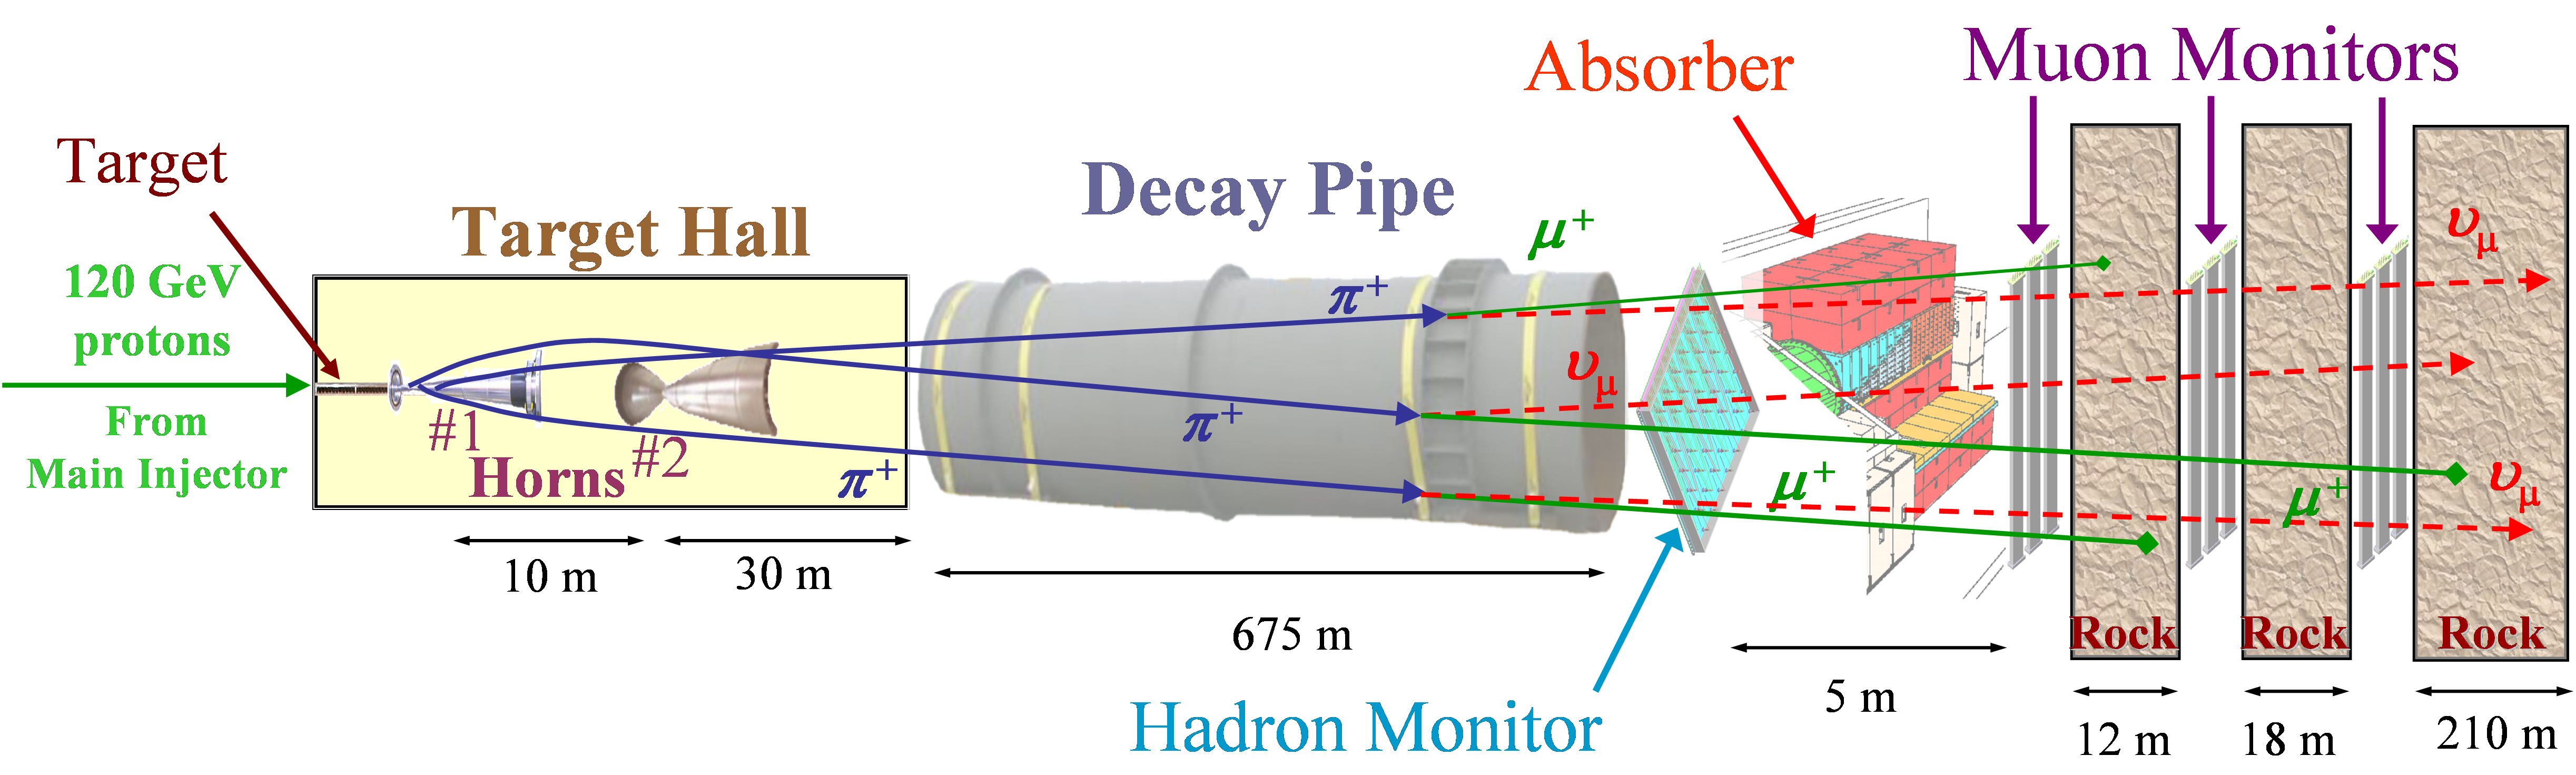
\includegraphics[width=1.0\textwidth]{figures/Beamline.png}
\centering
\caption{Schematics of neutrino production\cite{numi}.} \label{fig:NuMI}
\end{figure}
Neutrinos for the NOvA experiments comes from decay of pions and kaons. To get a beam of 
meson the Main Injector at Fermilab is used, which provides an intense beam of proton with 
energy 120 GeV. The structure of NuMI is illustrated on figure \ref{fig:NuMI}. It is designed to 
deliver $4.9 \times 10^{13}$ proton on target (POT) with the repetition rate of 1.3s, which 
corresponds to 700 kW of beam power. The proton beam is directed into a graphite target.  
Collisions between the proton beam and graphite target produces many types of hadrons and 
mesons, with pions and kaons among them. Magnetic focusing horns, which are supplied with 
current of 200kA, are used to focus and direct 
charged pions and kaons into a decay pipe. The decay pipe is long enough such that more than 
99\% of all pions 
and 63\% of kaons decay into anti-muon/muon and muon/anti-muon neutrino, so the flux of 
particles at the end of the decay pipe consists of mostly muons and muon anti-neutrinos, or 
their antiparticles. By changing the electric current direction in the focusing horns one can 
switch between focusing positively or negatively charged pions and kaons into the decay pipe. 
This gives an opportunity to make two types of neutrino beams - $\nu_\mu$'s and $\bar{\nu}_\mu$'s. 
Unfortunately, 5\% of charged kaons and muons, those which decay in decay pipe, have electron neutrinos 
among their byproducts, and this is an irreducible background for an electron neutrino analysis. 
The rest of charged particles such as undecayed muons and electrons do not reach Near Detector as they 
get absorbed in rock. A hadron monitor, absorber and muon monitor are placed at the end of decay pipe 
to better understand beam properties, but they do not play any role in the NOvA experiment.

\begin{wrapfigure}{r}{0.5\textwidth}
\vspace{-20pt}
  \begin{center}
    \includegraphics[width=0.48\textwidth]{figures/Neutrino_osc.png}
  \end{center}
\vspace{-30pt}
\caption{Neutrino oscillation probabilities.}
{Neutrino oscillation probabilities as a function of $\frac{L}{E}$, $P(\nu_\mu \rightarrow \nu_\mu)$ - 
blue line, $P(\nu_\mu \rightarrow \nu_e)$ - black line and $P(\nu_\mu \rightarrow \nu_\tau)$ - red line.}
\end{wrapfigure}

After the neutrinos leave the decay pipe they begin their journey to the near and far detectors.
The NO$\nu$A detectors are placed 14.6 mrad off-axis of the NuMI beam for several reasons. As can
be seen on the picture on the right, the first minimum of the muon neutrino survival
probability and first maximum of the electron neutrino appearance probability occur near 400 km/GeV. 
%To get a better 
%$\delta_{CP}$ sensitivity neutrino baseline should be as big as possible and for the practical reasons
%baseline is choosen to be 810 km. 
For this baseline of 810 km $P(\nu_\mu \rightarrow \nu_e)$ corresponds
to 2 GeV of neutrino energy. Only a tiny fraction of neutrinos satisifies this condition if Far Detector 
stays on-axis of neutrino beam as shown in Figure \ref{fig:Spec} and 
there should be a way to fix that. The solution is simple: pions and kaons decay isotropically in their 
rest frame, but, after a Lorentz boost to the laboratory frame, the neutrino flux and energy at the Far 
Detector (for small off-axis angles $\theta$) can be expressed in the following form
\be
F = \Big(\frac{2\gamma}{1+\gamma^2\theta^2}\Big)^2\frac{A}{4\pi d}
\ee
\be
E_\nu = \frac{0.43E_\pi}{1+\gamma^2\theta^2},\label{EnuvsEpi}
\ee
where $\gamma = \frac{E_\pi}{m_\pi}$, $A$ is the size of the detector front area and $d$ is 
the distance to the detector. For kaons numerical factor $0.43$ should be changed to $0.96$. 
Knowing the pion and kaon energy spectrum at the NuMI source, the neutrino energy spectrum at
the far detector for different off-axis angles $\theta$ can be predicted. As shown on the top of
figure \ref{fig:Spec}, as $\theta$ increases the neutrino energy distribution gets narrower and shifts
toward lower energies. At 14.6 mrad the neutrino flux is still appreciable and peaks near 2 GeV.
Based on this configuration, the NOvA Far Detector is situated 810 km from the source to measure
the maximum of $P(\nu_\mu \rightarrow \nu_e)$. At this distance, the narrow peak decreases the
probability that neutral current (NC) events from more energetic neutrinos are misidentified
as CC events in the energy region of interest\footnote{For example, a 10 GeV neutrino after NC interaction
can still have 8 GeV of energy and the rest of the energy si deposited in the detector as visible energy.}. 
In general, the off-axis detector placement significantly improves the sensitivity of the 
$P(\nu_\mu \rightarrow \nu_e)$ probability measurement.
\begin{figure}
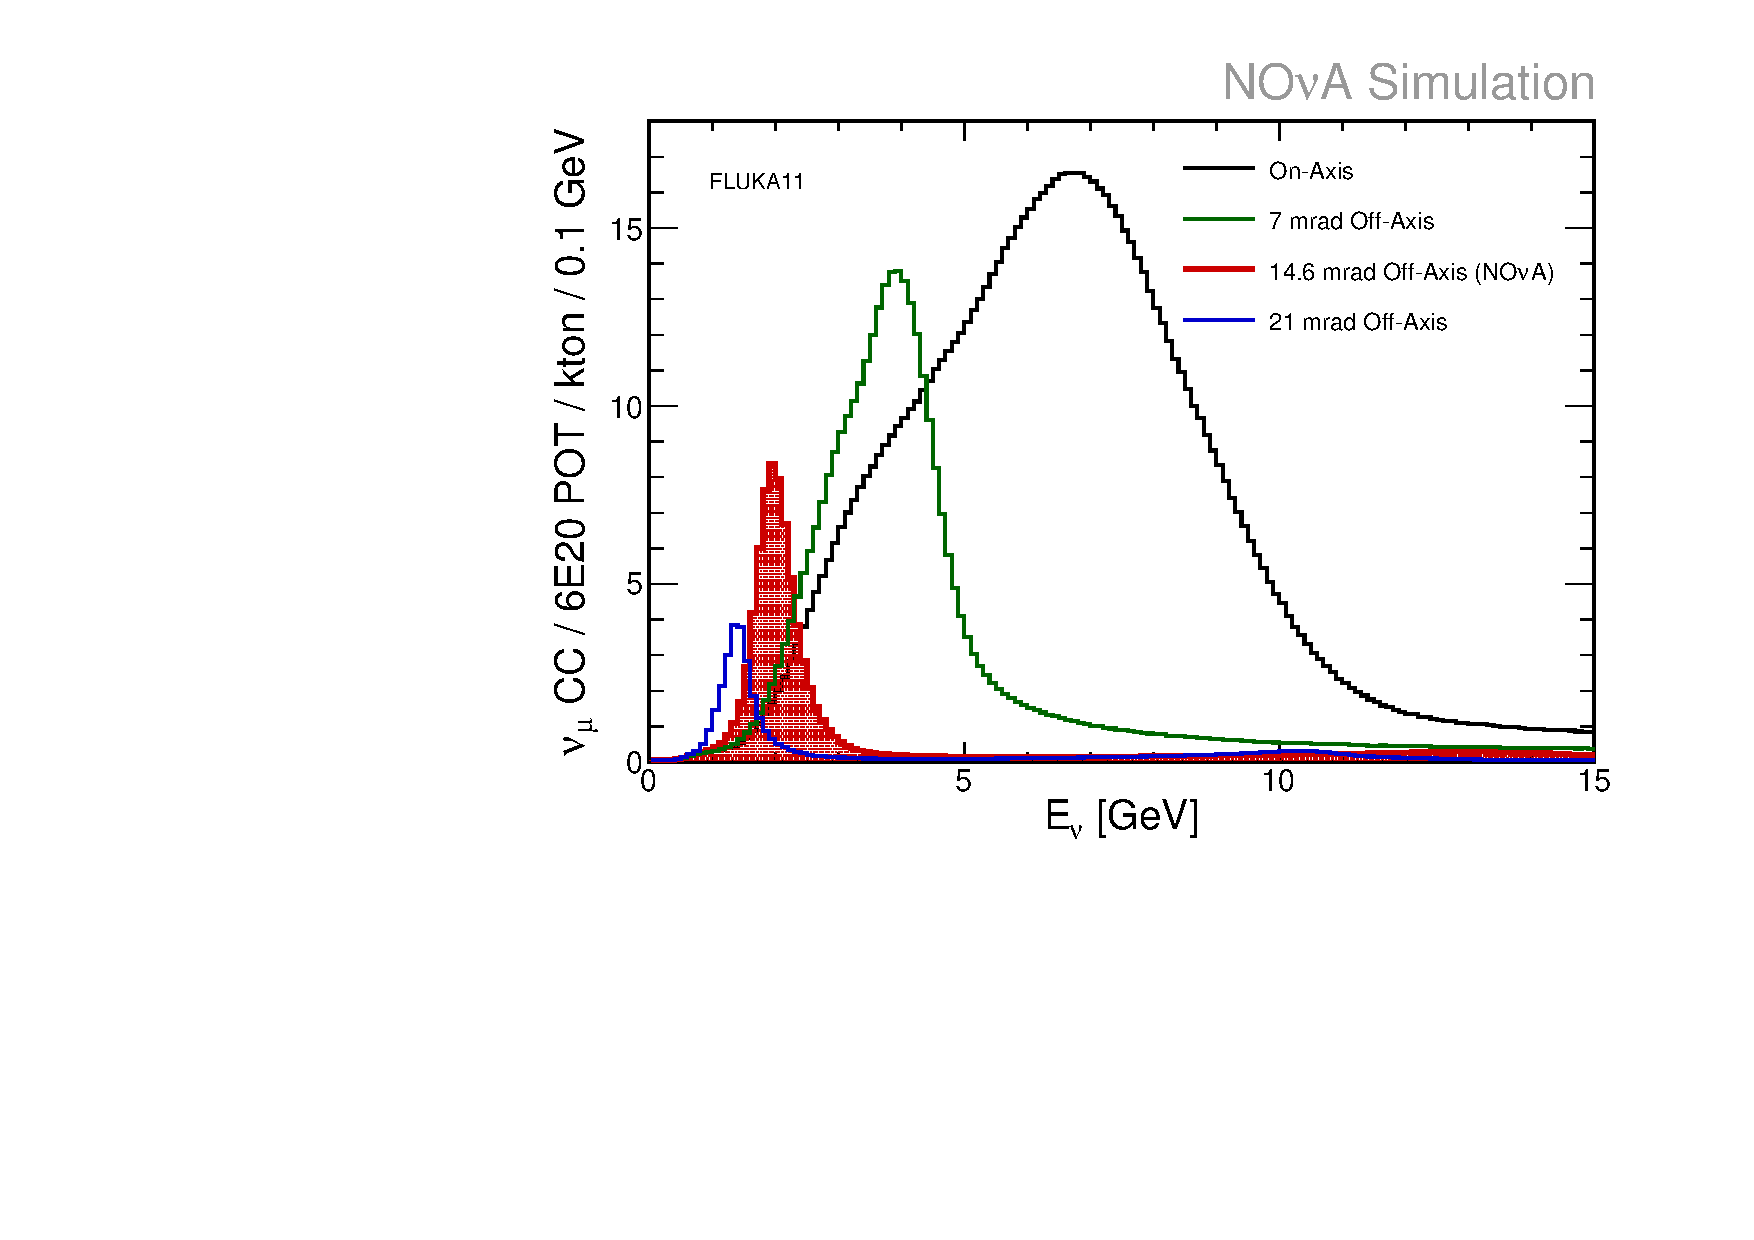
\includegraphics[width=0.9\textwidth]{figures/FD_NOvA_OffAxis_Spectra.pdf}\\%
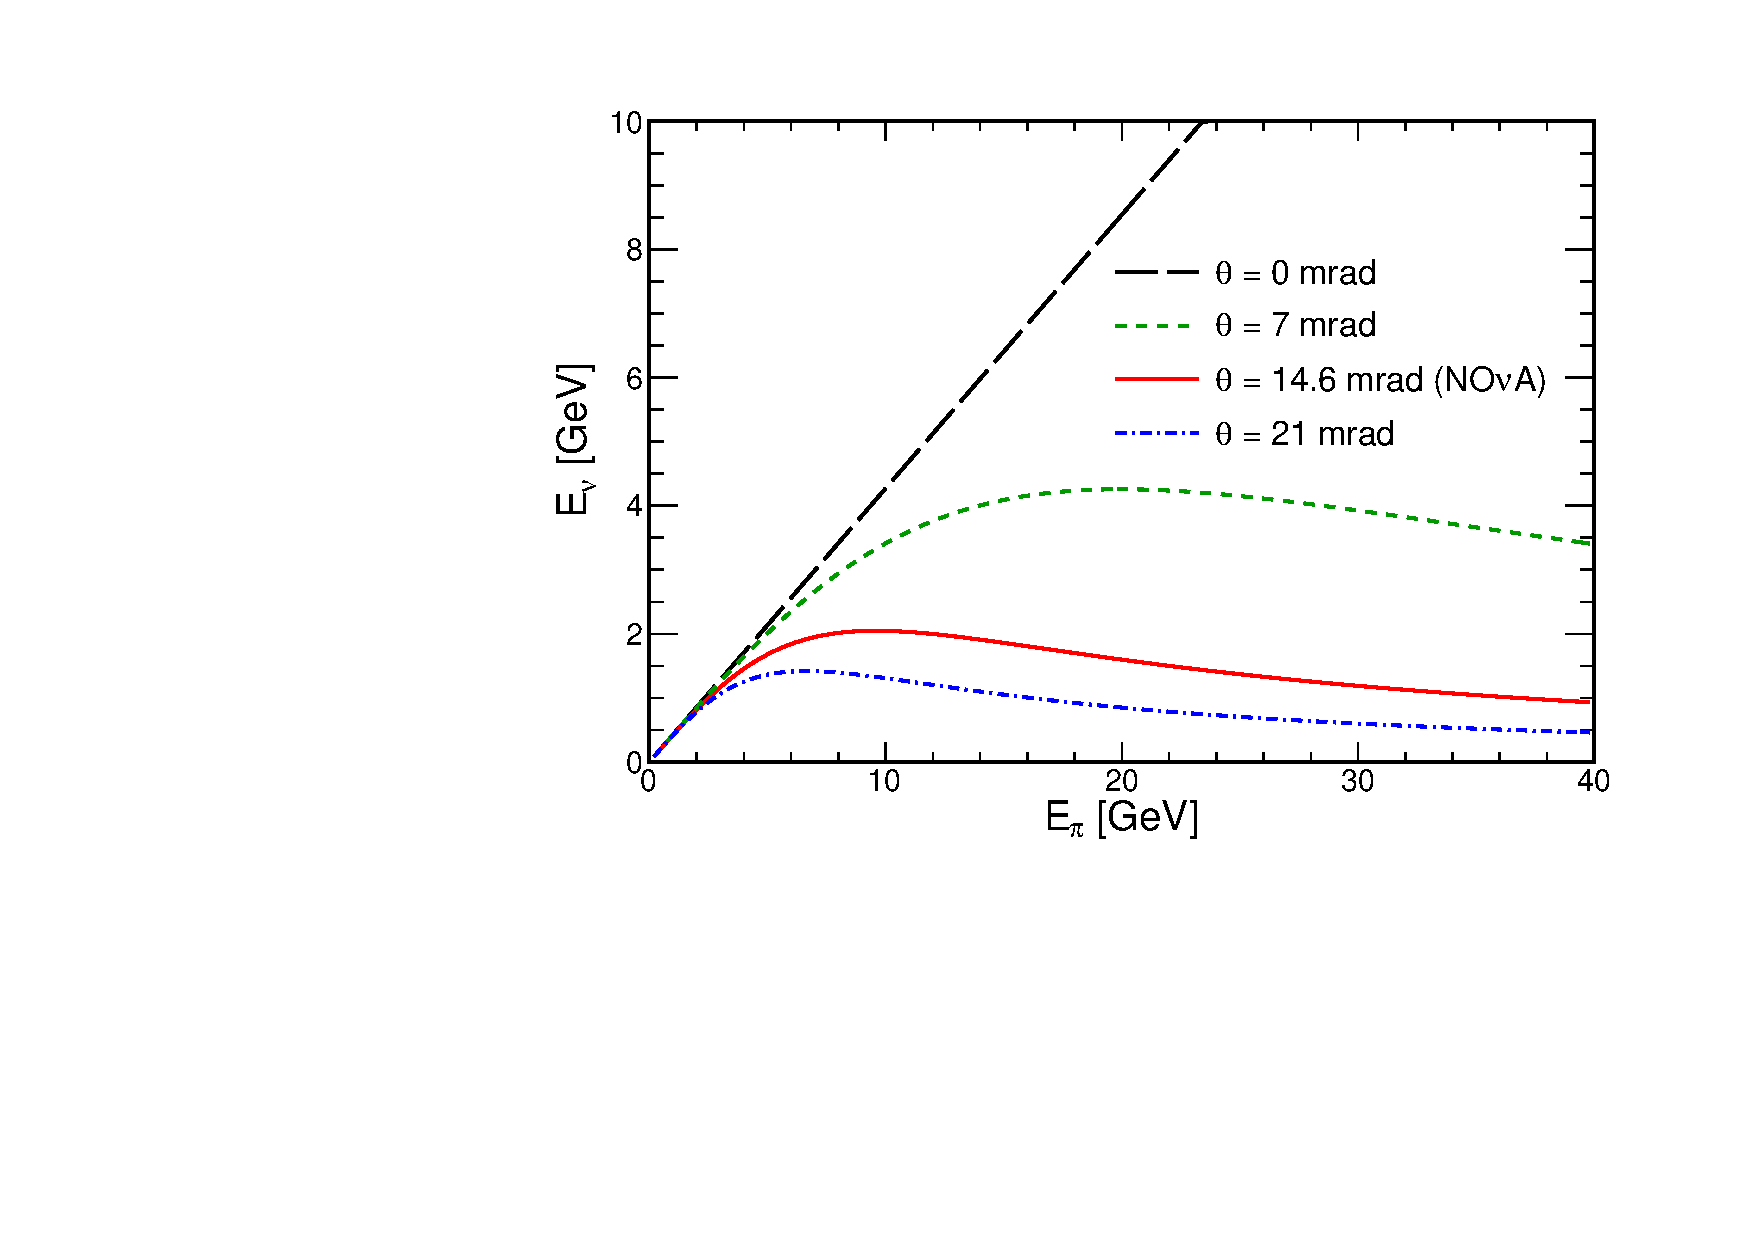
\includegraphics[width=0.9\textwidth]{figures/EnuVSEpi_NOvA.pdf}
\centering
\caption{(Top) Expected unoscillated neutrino spectrum at the Far Detector as a function of 
angle relative to NuMI beam. (Bottom) Neutrino energy as function of pion energy (eq. \ref{EnuvsEpi}) 
for different off-axis angles.} \label{fig:Spec}
\end{figure}

\section{NOvA Near and Far Detectors}
The NOvA experiment uses two detectors for measuring muon neutrino disappearance probability 
$P(\nu_\mu \rightarrow \nu_\mu)$ and electron neutrino appearance probability $P(\nu_\mu \rightarrow \nu_e)$. 
In order to decrease systematic uncertainties, such as beam uncertainty and uncertainties due to variation
in detector efficiency, two detectors are built with exactly the same material and 
similar technology. The Near Detector is placed 1 km from the NuMI source at Fermilab, while the 
Far Detector sits 810~km away on the surface and 14.6 mrad off beam axis in Ash River, Minnesota. 
The Near Detector weighs 330 metric ton and is 105 m underground, while the Far Detector mass is 
14,000 ton and has shielding equivalent to 3 m of water which reduces cosmic ray background.
The reason the Near Detector is underground is that on the ground NuMI source has to shoot the neutrino beam 
approximately 3.6 degrees below the ground level so it comes out of the Earth 810 km downrange. 
\begin{figure}
\begin{subfigure}{.2\textwidth}
  \centering
  \includegraphics[width=0.79\linewidth]{figures/PVC_cell_original.jpg}
  \caption{A NOvA cell}
  \label{fig:cell}
\end{subfigure}%
\begin{subfigure}{.8\textwidth}
  \centering
  \includegraphics[width=\linewidth]{figures/2detectors.pdf}
  \caption{Scale and structureof the NOvA detectors}
  \label{fig:2detectors}
\end{subfigure}
\caption{Structure of cell and the NOvA detectors}
\label{fig:cell_detectors}
\end{figure}

\subsection{Internal construction}
Each detector is made of cells which are made from polyvinyl chloride (PVC) doped with titanium 
dioxide to increase light reflectivity. The cross section of cells has rectangular shape with sizes
approximately equal to 4 cm and 6 cm. The length of the cells are varies between the detectors and 
is 4 m for the Near Detector and 15 m for the Far Detector. 32 cells are bound together along
6 cm side to make a module and a set of modules produces plane. The number of modules in a plane
depends on a detector - 3 and 12 modules per plane for the Near and Far Detector respectively. Planes
are glued together in a such way that adjacent planes alternating between horizontal and vertical
allignment. The scetch of the detectors structure can be seen in \ref{fig:2detectors}. Furthemore, 32 planes 
make up a block and 28 blocks complete the full Far Detector while for the Near Detector block consists
of 24 planes and 3 blocks make the active part of the detector. In addition, so-called muon catcher
block goes downstream of the Near Detector and serves for stopping muons which are produced in $\nu_\mu$ 
CC interactions. The muon catcher, which helps to contain more muons as the relative size of the Near 
Detector is not big, consists of 22 active planes, with ten steel planes of 10 cm thickness interspersed 
between pairs of active planes. The size of the muon catcher in the XY plane is smaller the the active 
part of the Near Detector. The steel absorbs additional particle energy, and results in shorter muon tracks.

Using the planes configuration, three-dimensional particle tracks are reconstructed: vertical planes
provide X measurements, horizontal planes provide Y measurements, and the Z measurements are extracted from
the plane positions. The Z-axis is directed along the beam, the X-axis points to the west and the Y-axis points
upward. This choice of axes results in a Cartesian right handed coordinate system.

\subsection{Light production and digitization}
In order to detect particles resulted in neutrino interactions in the detectors these particles 
should leave footprints. In NOvA experiment cells are filled with a liquid scintillator composed 
of mineral oil doped with pseudocumene~\footnote{1,2,4-Trimethylbenzene}. In every cell, one wavelength 
shifting fiber runs from one end of the cell to the opposite end, then back to the other end where 
it connects to an avalanche photodiode (APD) as can be seen in \ref{fig:cell}. Photons are created by charged 
particle moving through the scintillator. These reflected by the cell walls and have a high chance 
to be captured by the wavelength shifting fiber. Inside the fiber photons after absorbtion and
reemission increase its wavelength resulting in propogation without escaping due to total inner
reflection. 

Photons that reach each APD are converted into a current of photoelectrons through the avalanche breakdown 
process. All 32 fiber of each module are connected to one APD. And the last step before signals might be 
processed with the 
help of conventional computers is to digitize the APD output signal. The digitization happens in
front end board (FEB). Short APD signals are stretched in time in the Application Specific 
Integrated Circuit (ASIC) with the help of CR-RC circuit. After, the signal is passed to ADC - 
analog to digital converter - where continuous signal is converted to discrete, 12-bit signal
that is read out every 500 (125) ns at the Far (Near) Detector, respectively. Only the 4 first ADCs - 
value of the digitization sample - are stored as a hit and the hit is written when the difference
\be
ADC_i - ADC_{i-3}
\ee
is greater than a threshold. These 4 values are then passed to the Data Concentration Module (DCM). 
Later, those 4 values are used to fit the signal shape and to determine signal amplitude, which 
is proportional to amount of energy charged particle deposited in a particular cell.

\subsection{Data acquisition}
Every DCM is a custom built computer and collecting data from 64 FEBs. Data from the FEBs
is sorted in time and arranged into 5 ms data blocks, then the data is sent to a buffer node where it 
is stored until a trigger decision is made to save the data permanently to the disks. 200 buffer nodes 
are arranged in a circular ring buffer and every node has up to a minute to run a trigger software 
until a new piece of data comes from a DCM. NOvA trigger software which issues trigger decisions relies
on external triggers as well as data-driven triggers based on received data. Neutrino oscillation
analyses use data which are recorded due to a timing trigger, this so-called NuMI trigger 
is issued by the acceleration complex at Fermilab. The trigger records 550 $\mu s$ window of data centered 
around the 10 $\mu s$ NuMI beam spill. There are several more triggers such as a cosmic trigger, which 
triggers at the rate of 10 Hz to store FD cosmic data for callibration and background estimation, and a 
supernova trigger, which should record up to 1 minute of data in the event of supernova burst.

The data selected by the triggers is stored temporarily at the FD and ND sites, and eventually transferred
to Fermilab where it is processed for further analysis.

\subsection{Neutrino Interactions in NOvA}
\begin{figure}
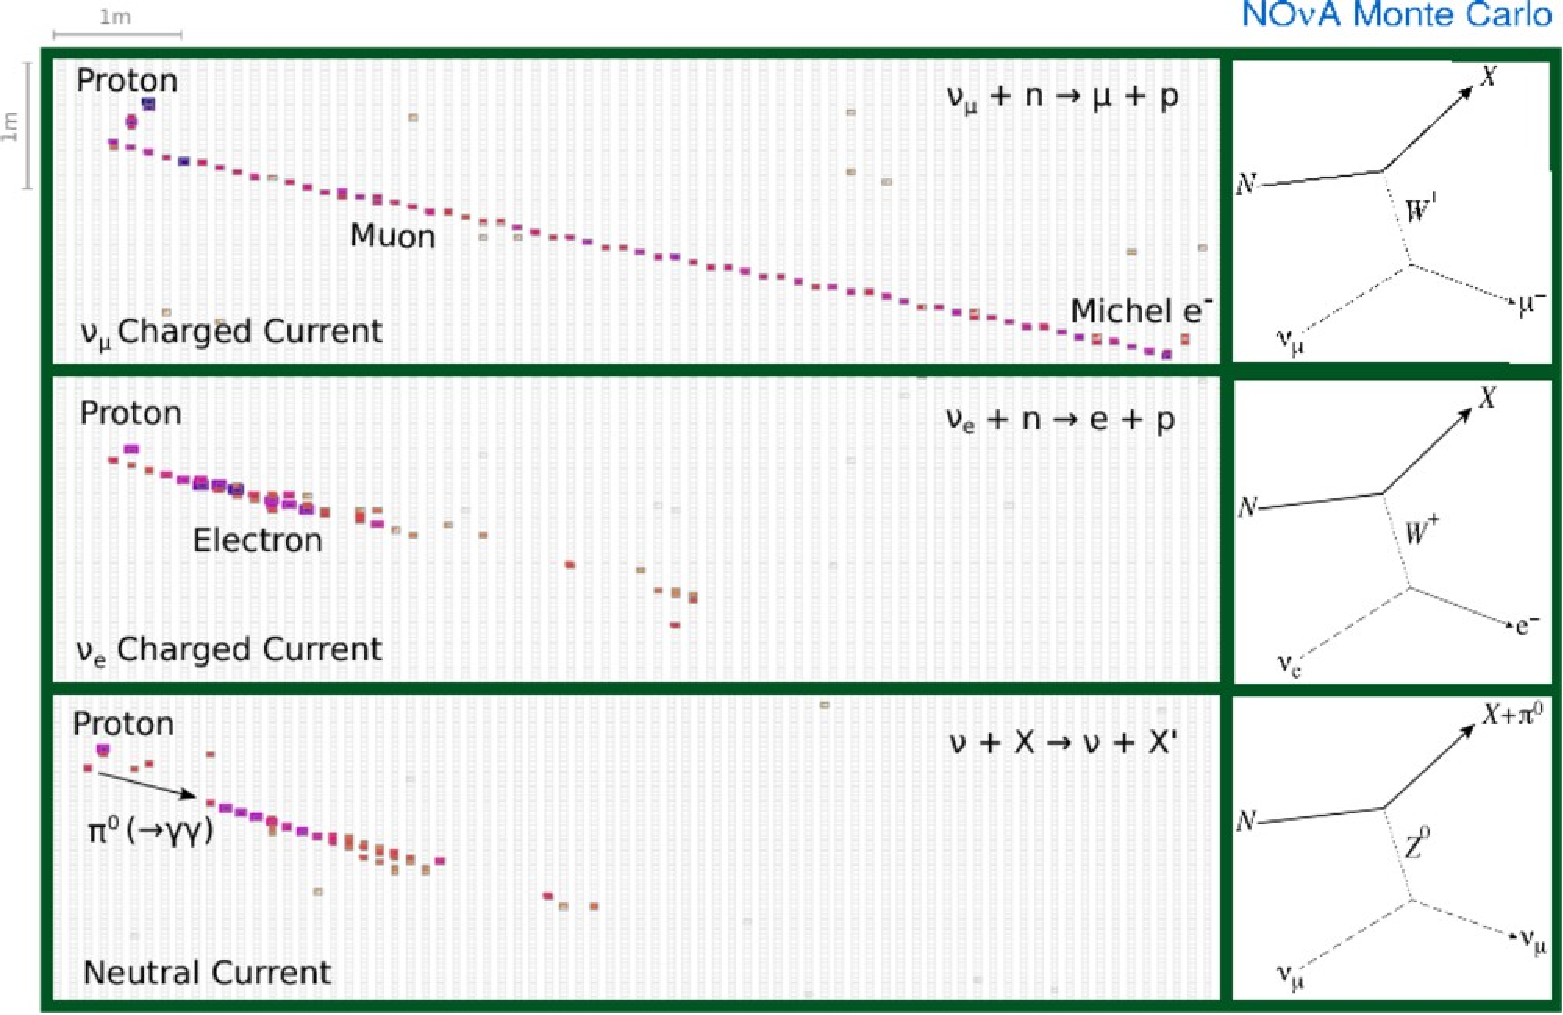
\includegraphics[width=1.0\textwidth]{figures/Det_topologies.pdf}\\%
\caption{Neutrino interactions in NOvA detectors.}
{Three types of neutrino interactions are shown. The top part shows $\nu_\mu$ CC interaction with some
proton activity and long muon track left by high energy muon. The middle part shows $\nu_e$ CC interaction,
electron develops a long electromagnetic shower with radiation length being much bigger than Moliere radius.
The bottom part shows neutrino NC interaction with $\pi^0$ among the resulting particles which later produces
an electromagnetic shower by decaying into two photons. NC type events form a primarily background in $\nu_e$
disapperance analysis.} \label{fig:Topologies}
\end{figure}
The majority of neutrinos impinging on the NOvA detectors carry a few GeV energy, and all the charged
products of a neutrino-nucleon interaction are clearly visible and can be individually tracked as long as their 
trajectories are sufficiently separated. As illustrated in figure \ref{fig:Topologies} muons, electrons, 
and neutral pions produce a distinct signatures in NOvA. Particles primary lose their energy through an 
ionization 
process by disrupting electrons of atoms which happen to be close to particles trajectories. Being 
much heavier than an electron and immune to a strong interaction a muon can travel a long distance
\footnote{Approximately 4.5 meters per 1 GeV of muon energy} inside the detectors which make it a relatively 
easy task to determine a high energy muon. Electrons interact with detector material electromagnetically, and 
quickly shower energy in a small conical region as opposed to a long muon track. Hadrons such as protons and 
charged pions lose energy through ionization and strong interactions with nucleons along their trajectories, and tend 
to travel much shorter distances than muons.

Despite these differences it is a complicated problem to distinguish a charged current (CC) interaction with
a muon or electron being produced from a neutral current (NC) interaction where no visible lepton is produced.
NC processes can produce charged or neutral pions with other hadrons. Charged pions
leave tracks which could be confused with low energy muons, although occasional hard scatters with 
nuclei help with identification. Neutral pions decay into two photons and produce electromagnetic
showers, and these showers can be mistaken with showers from electrons in CC interactions.
Thus, sophisticated algorithms were developed to determine the exact neutrino flavor.

In addition, since the NOvA Far Detector sits on the ground it is constantly being bombarded by muons and other
particles created by interactions of cosmic rays with air molecules in upper atmosphere. 
These muons contribute to a background for the main analysis but they are relatively easy to get rid off
because of their activity at the top and/or at the sides of the detector and main analysis consider activity 
which is fully contained in the detector volume. However, cosmic muons are a primarily background in a escaping 
sample which this thesis is partially about.

\subsection{NOvA Event Display}
\begin{figure}
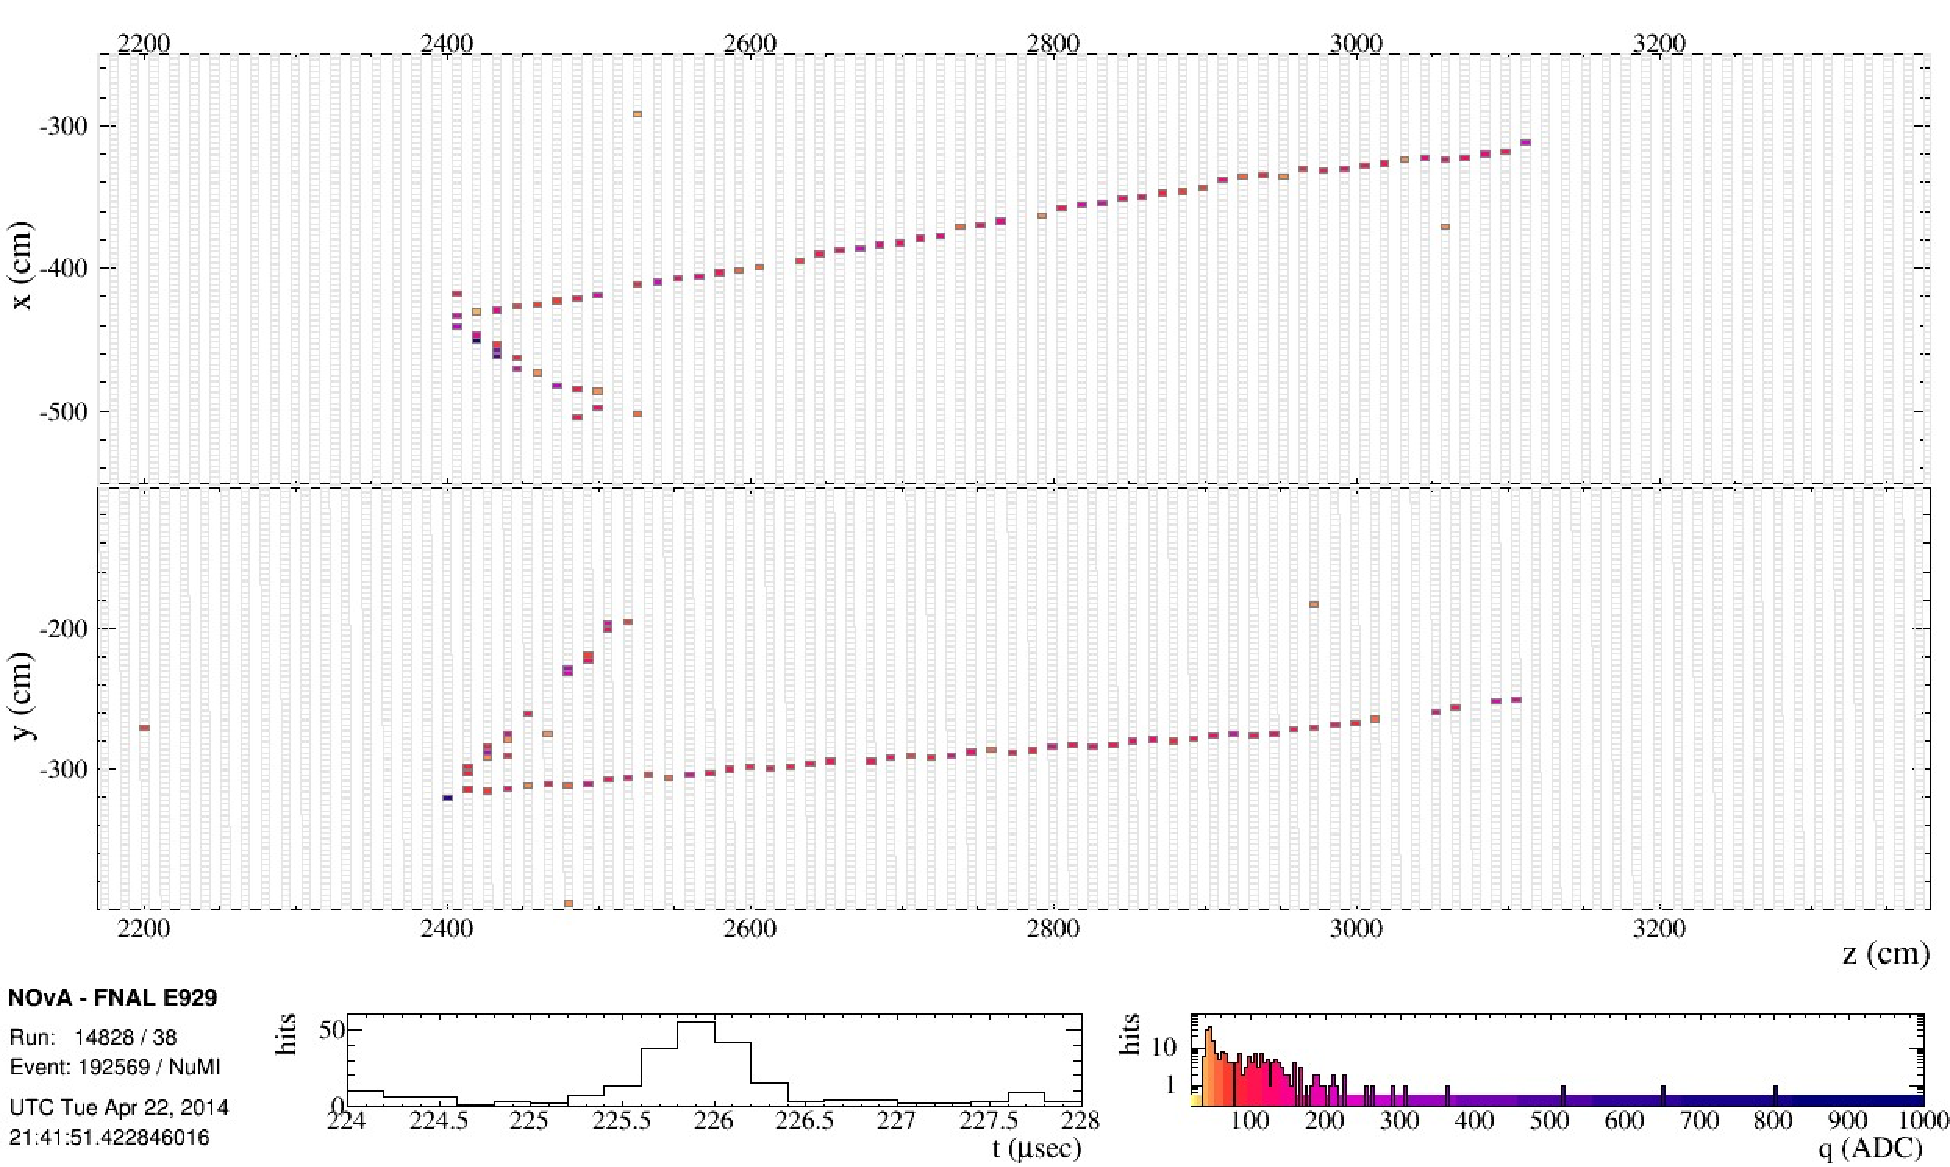
\includegraphics[width=1.0\textwidth]{figures/EventDisp.pdf}\\%
\caption{NOvA Event Display.}
{The candidate $\nu_\mu$ CC event at the Far Detector zoomed in space and time. Top and bottom windows show
X-Z and Y-Z projections.} \label{fig:EVD}
\end{figure}
The NOvA event display helps to visualize data gathered by the detectors or a simulated one. The result
of $\nu_\mu$ CC interaction measured on April 22, 2014 is shown in \ref{fig:EVD}. As NOvA detectors consist of 
alternating horizontal and vertical planes, event display shows hits from two types of planes in a separate 
windows. The top window displays X-Z hits position (detector activity as seen from the top), while the lower 
one displays Y-Z hits position (detector activity as seen from the side). The software allows to change a spatial zoom as well as a time zoom to see closely activity he/she might be interested in. Hits time distribution and 
deposited photoelectron charge distribution in ADC units together with event time stamp and trigger information 
are shown below the main windows. Hits also could be colored by their time, to see if they are close to readout 
window or not, or by their deposited charge, to see where the most of the energy was deposed. In the shown 
example, hits are colored by their charge.
